\documentclass[12pt,a4paper]{scrartcl}
\usepackage[utf8]{inputenc}
\usepackage[english,russian]{babel}
\usepackage{amssymb,amsfonts}
\usepackage{amsmath,cite,enumerate}
\usepackage{float,indentfirst}
\usepackage{graphicx}
\usepackage{geometry} % Меняем поля страницы
\geometry{left=2cm}% левое поле
\geometry{right=1.5cm}% правое поле
\geometry{top=1cm}% верхнее поле
\geometry{bottom=2cm}% нижнее поле
\graphicspath{{images/}}

\begin{document}


\begin{titlepage}
  \begin{center}
    Санкт-Петербургский Политехнический Университет     Петра Великого \\
    
    Институт компьютерных наук и технологий \\
    
    Кафедра компьютерных систем и программных технологий
  \end{center}
  
  \vfill
  
  \begin{center}
  Лабораторная работа №1, 2\\
  по теме\\
  "Сигналы телекоммуникационных
систем"\\
\end{center}

\vfill

\newlength{\ML}
\settowidth{\ML}{«\underline{\hspace{0.7cm}}» \underline{\hspace{2cm}}}
\hfill\begin{minipage}{0.4\textwidth}
  Выполнил студент группы 33501/3\\
  \underline{\hspace{\ML}} Ромащенко Д.\,Ю\\
\end{minipage}%

\bigskip

\settowidth{\ML}{«\underline{\hspace{0.7cm}}» \underline{\hspace{2cm}}}
\hfill\begin{minipage}{0.4\textwidth}
  Руководитель\\
  \underline{\hspace{\ML}} Богач Н.\,В\\
\end{minipage}%

\vfill
 
\begin{center}
  Санкт-Петербург\\
2018 
\end{center}

\end{titlepage}

\section{Цель}
\label{sec:goal}

Познакомиться со средствами генерации сигналов и визуализации их спектров.\\

\section{Постановка задачи}
\label{sec:task}

В командном окне MATLAB и в среде Simulink промоделировать синусоидальный и прямоугольный сигналы с различными параметрами. Получить их спектры. Вывести на график.\\

\section{Теоретический раздел}
\label{sec:teoriya}
\textbf{Гармонические} сигналы, записываются следующим способом:
$$s(t)=A\cos (\omega t+\varphi _0),$$ где  A - амлитуда колебаний, $\omega$ - циклическая (круговая) частота, $\varphi _0$ - начальная фаза, $\varphi = \omega t+\varphi _0$ - фаза колебаний.


\textbf{Меандр} - это прямоугольный сигнал, у которого длительность импульса и паузы равны. Обычный прямоугольный сигнал отличается от меандра тем, что имеет разную длительность импульса и паузы. 

\begin{figure}[h!]
\center{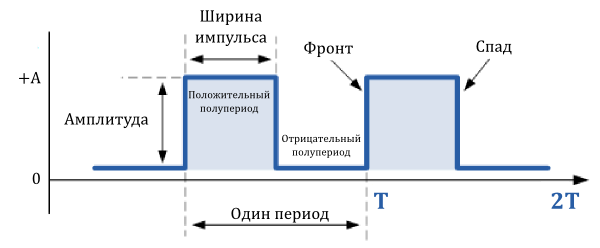
\includegraphics[width=0.6\linewidth]{teoria_pryam_signal}}
\caption{Параметры прямоугольного сигнала}
\end{figure}

Прямоугольные сигналы можно охарактеризовать \textbf{скважностью} (S) и \textbf{коэффициентом заполнения} (D):

$$S=\frac{T}{\tau}=\frac{1}{D}$$

Совокупность амплитуд гармоник ряда Фурье часто называют \textbf{амплитудным спектром}, а совокупность их фаз - \textbf{фазовым спектром}.

Разложению в ряд Фурье могут подвергаться периодические сигналы. При этом представляются в виде суммы гармонических функций либо комплексных экспонент с частотами, образующими арифметическую прогрессию. Для того, чтобы такое разложение существовало, фрагмент сигнала длительностью в один период должен удовлетворять условиям Дирихле:\\
1) Не должно быть разрывов второго рода ( с уходящими в бесконечность ветвями функциями);\\
2) Число разрывов первого рода (скачков) должно быть конечным;\\
3)Число экстремумов должно быть конечным.

Комплексная форма записи ряда Фурье:
$$s(t)=\sum_{k=-\infty}^\infty C_k e^{-jk\omega t}$$

Комплексные коэффициенты ряда связаны с амплитудами $A_k$ и фазами $\varphi _k$, фигурирующими в вещественной форме записи ряда Фурье, следующими соотношениями:

$$C_k = \frac{1}{2}A_k e^{j\varphi k},$$

$$A_k = 2|C|_k|$$

Формула прямого преобразования Фурье:

$$S(\omega) = \int_{-\infty}^\infty s(t) e^{-j\omega t} dt$$

Чтобы преобразование Фурье было применимо, сигнал должен удовлетворять следующим требованиям:

1) должны выполняться условия Дирихле;\\
2) сигнал должен быть абсолютно интегрируемым. Это означает, что интеграл от его модуля должен быть конечной величиной:

$$\int_{-\infty}^\infty|s(t)|dt<\infty$$

Однако с привлечением математического аппарата обобщенных функций возможно выполнение Фурье-анализа и для некторых сигналов, не удовлетворяющим этим требованиям.
\\


\section{Ход работы}
\textbf{Построение синусоидального сигнала и его спектра в командном окне Matlab:\\}

Текст программы:\\
\\
ts=0.01 \% задаем частоту дискретизации\\
t = 0:ts:2*pi; \\
N = 512;\\
f0 = 10;\\
\% исходный сигнал\\
y = sin(2*f0*pi*t);\\
plot(t(1:200),y(1:200)) \\
grid\\
\% спектр исходного сигнала\\
figure\\
\% прямое преобразование Фурье\\
plot(abs(fft(y, N)))\\

Результат работы программы - на рис.1 и 2\\
\begin{figure}[h!]
	\center{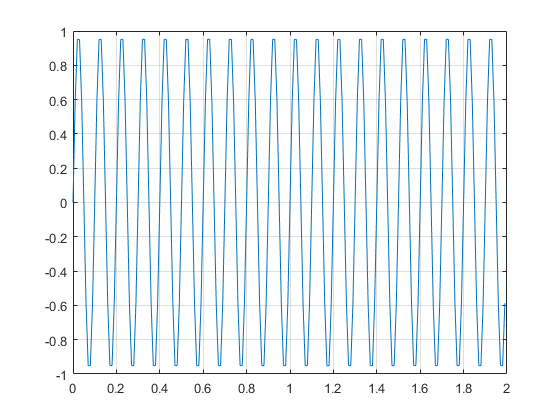
\includegraphics[width=0.6\linewidth]{Sin_signal}}
	\caption{Синусоидальный сигнал.}
\end{figure}
\begin{figure}[h!]
	\center{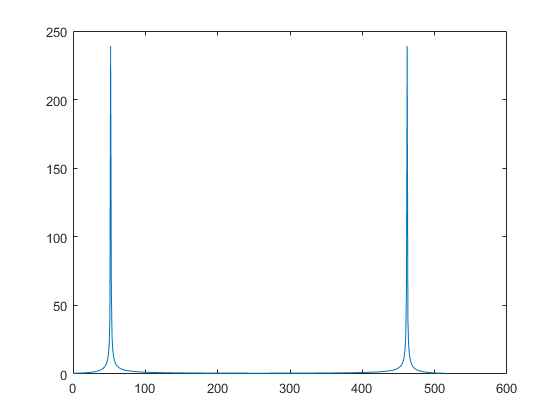
\includegraphics[width=0.6\linewidth]{Sin_spectr}}
	\caption{Спектр синусоидального сигнала.}
\end{figure}
\newpage
\textbf{Построение прямоугольного сигнала и его спектра в командном окне Matlab:\\}

Текст программы:\\
\\
tau=5*10\^(-3); \\
q = 5; \% скважность\\
n=1024;\\
Tp=tau*q;\\
N=6;\% число импульсов\\
T=N*q*tay; \\
Ts=T/(n-1);\\
d=(0:N-1)*Tp;\% вектор задержки \\
t=0:Ts:T; \\
A=5;\\
fd=(64*(2/q))/(q*tay);\\
\% исходная последовательность импульсов\\
s=A*pulstran(t,d,'rectpuls', tay);\\
figure;\\
plot(t,s);\\
x=A*rectpuls(t,tay);\\
x=A*2*x/(q*sum(x));\\
f=0:fd/n:fd/2-1/n;\\
X=fft(x,n);\\
Z=abs(X);\\
figure;\\
plot(f,Z(1:length(f))), xlim([0 3/(q*tay)])\\
\\
Результат работы программы - на рис.3 и 4\\

\begin{figure}[h!]
	\center{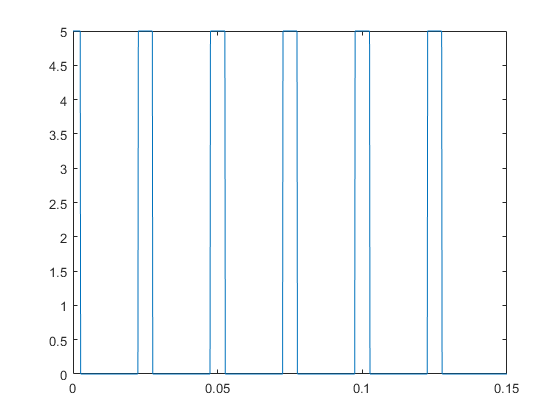
\includegraphics[width=0.6\linewidth]{Rect_signal}}
	\caption{Прямоугольный сигнал.}
\end{figure}
\begin{figure}[h!]
	\center{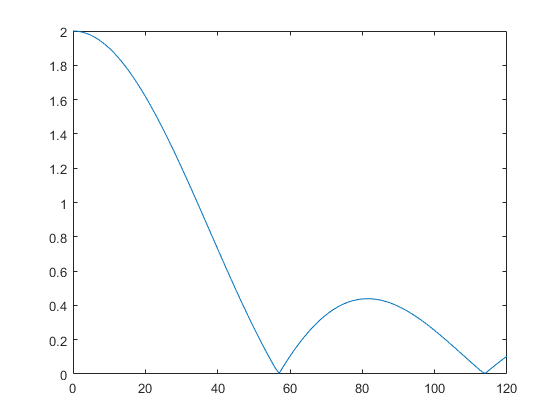
\includegraphics[width=0.6\linewidth]{Rect_spectr}}
	\caption{Спектр прямоугольного сигнала.}
\end{figure}
\newpage
\textbf{Построение синусоидального сигнала и его спектра в среде Simulink:\\\\}

Результаты работы - на рис. 6 и 7.
\begin{figure}[h!]
	\center{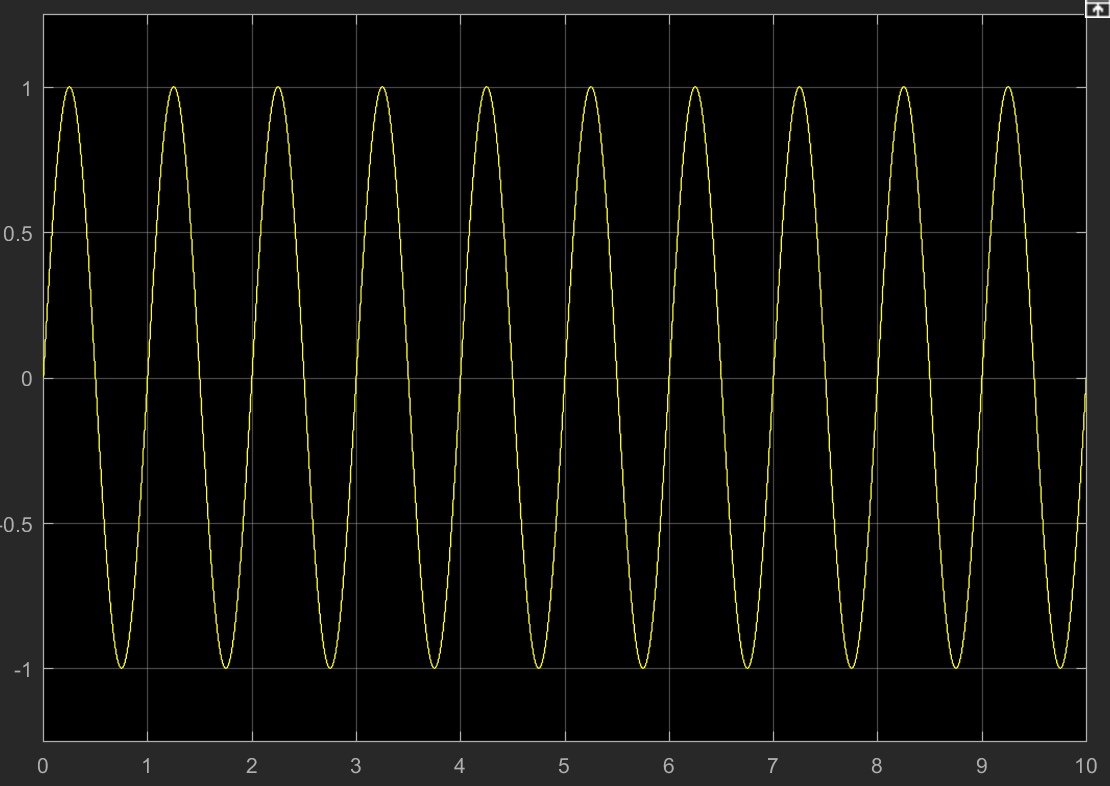
\includegraphics[width=0.6\linewidth]{Sin_signal_sim}}
	\caption{Синусоидальный сигнал.}
\end{figure}
\begin{figure}[h!]
	\center{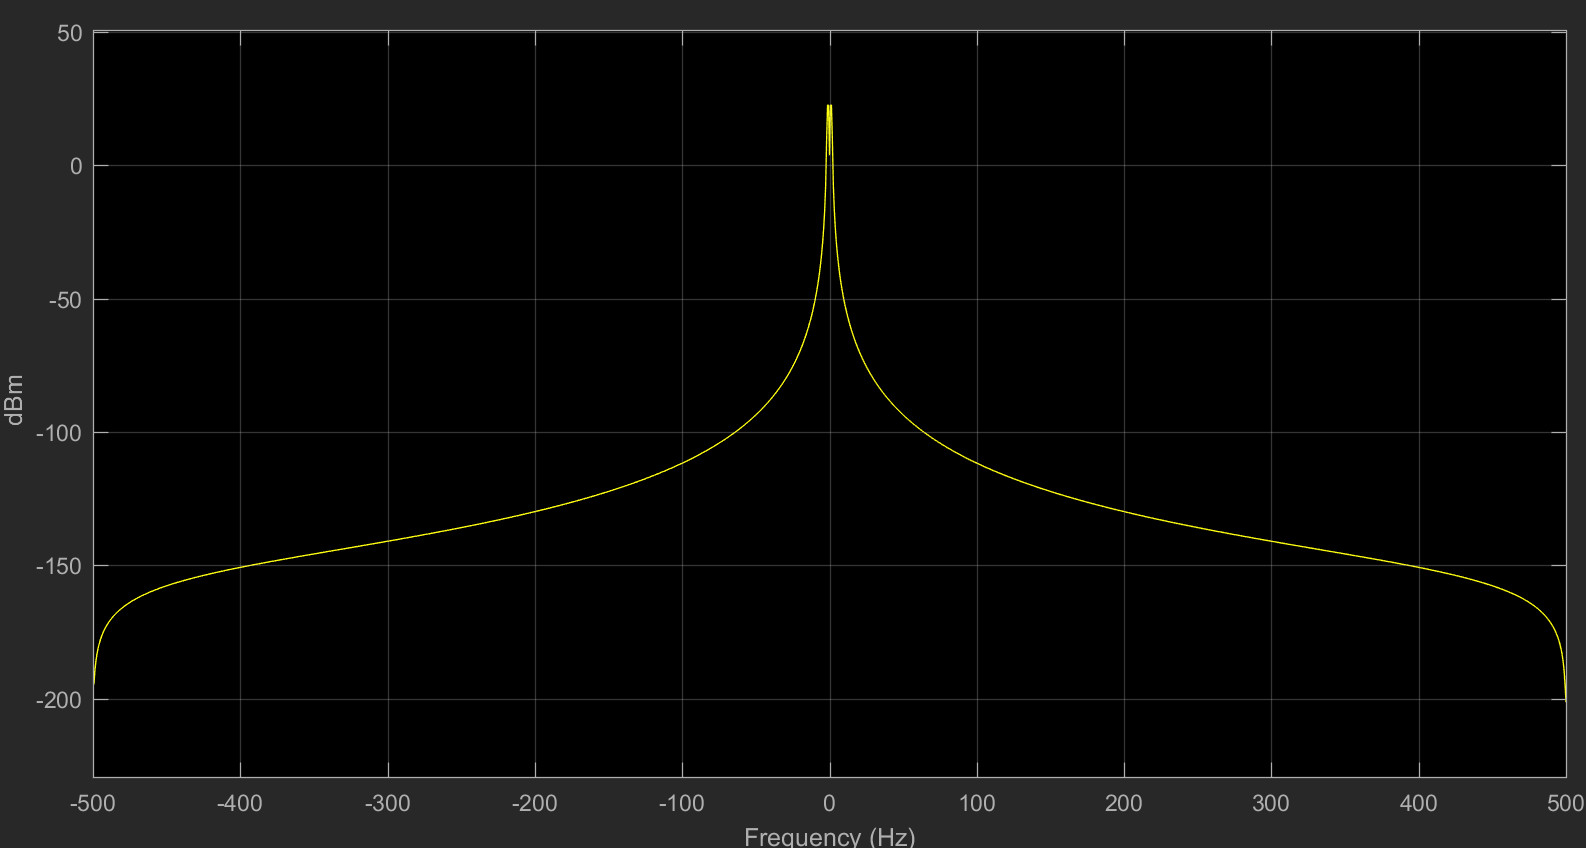
\includegraphics[width=0.6\linewidth]{Sin_spectr_sim}}
	\caption{Спектр синусоидального сигнала.}
\end{figure}
\newpage
\textbf{Построение прямоугольного сигнала и его спектра в среде Simulink:\\\\}

Результаты работы - на рис.9 и 10
\begin{figure}[h!]
	\center{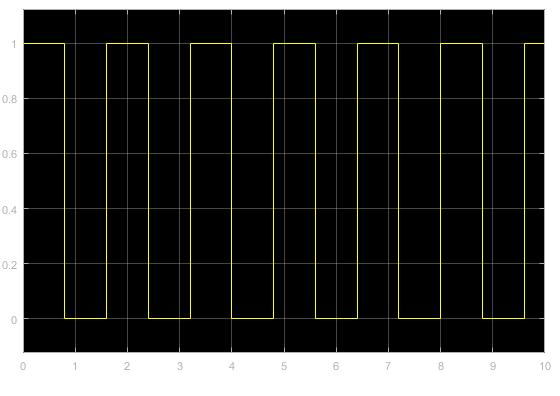
\includegraphics[width=0.6\linewidth]{Rect_signal_sim}}
	\caption{Прямоугольный сигнал.}
\end{figure}
\begin{figure}[h!]
	\center{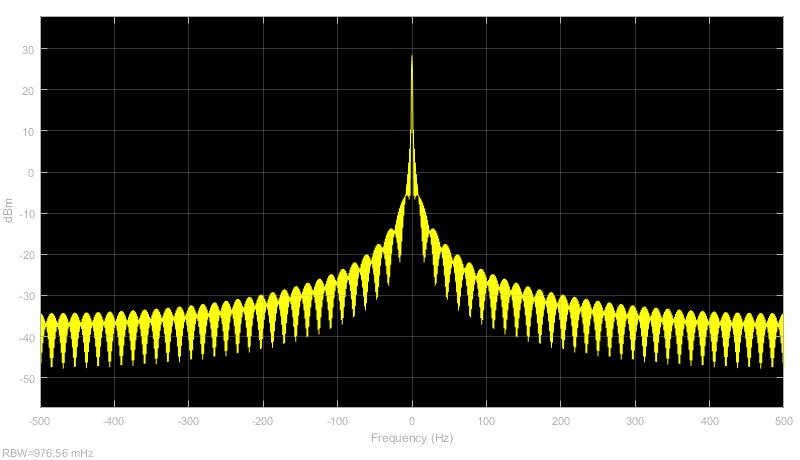
\includegraphics[width=0.6\linewidth]{Rect_spectr_sim}}
	\caption{Спектр прямоугольного сигнала.}
\end{figure}

\textbf{Корреляция :\\}
Есть дискретный сигнал [0001010111000010]. Необходимо найти позицию синхропосылки [101].
Позицию ссылки в сигнале можно найти с помощью функции корреляции : 
\begin{figure}[h!]
	\center{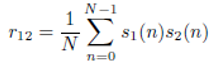
\includegraphics[width=0.3\linewidth]{Cor_fun}}
\end{figure}
\newpage
Максимальная корреляция будет соответствовать месту искомой посылки:
\begin{figure}[h!]
	\center{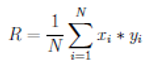
\includegraphics[width=0.2\linewidth]{Max_cor}}
\end{figure}

Быстрая корреляция:
\begin{figure}[h!]
	\center{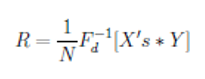
\includegraphics[width=0.2\linewidth]{Fast_cor}}
\end{figure}

Текст программы:\\
\\
close all;\\
x = [ 0 0 0 1 0 1 0 1 1 1 0 0 0 0 1 0 ];\\
y = [ 1 0 1 ];\\
figure;\\
tic;\\
CorrCross = xcorr(x,y);\\
time = toc\\
subplot(2,1,1)\\
plot(1:length(CorrCross),CorrCross);\\
tic;\\
Corrfast = ifft(fft(x).*conj(fft(y,16)));\\
time = toc\\
subplot(2,1,2)\\
stem(1:length(Corrfast),Corrfast);\\
\\

Время осуществления корреляции:\\  
0.00052 время выполнения прямой корреляции \\
0.00004- время выполнения быстрой корреляции \\

\begin{figure}[h!]
	\center{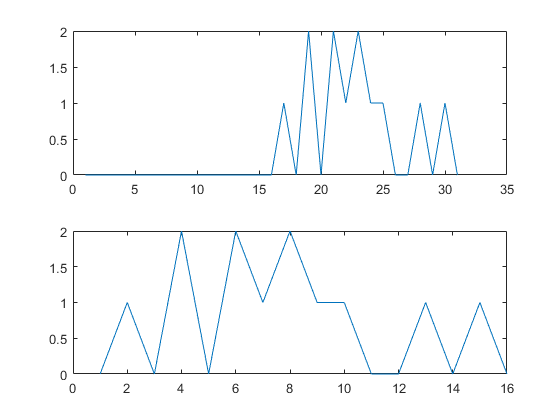
\includegraphics[width=0.6\linewidth]{Cor}}
	\caption{Результат корреляции.}
\end{figure}

\newpage
\section{Выводы}
В лабораторной работе были визуализированы синусоидальный и прямоугольный сигналы. Сигналы были созданы и анализированы в среде Matlab и Similink.

Все сигналы описываются набором параметров. Рассмотрим параметры изученных сигналов. Информационными параметрами гармонического сигнала являются амплитуда сигнала, фаза, период. Информационными параметрами прямоугольного сигнала яляются период повторения импульсов, длительность импульсов, скважность импульсов.

 Преобразование Фурье в телекоммуникационных технологиях используется для обработки звука и изображений. Примером использования преобразования Фурье является восстановление расфокусированного изображения. 
\end{document}